After thoroughly analyzing several iterations of prototypes and many rounds of 
brainstorming on specific aspects and features of gameplay and game components, 
the team designed a unified final prototype to develop in Unity. This unified prototype, 
shown in Figure \ref{fig:Unified_Prototype}, serves as the foundation for the game to 
be built on, so while many components will be added and changed throughout the 
development process, the overall game flow and mechanics will not deviate far from 
this prototype. The initial Unity prototype is shown in Figure \ref{fig:Unity_Prototype}.\\

\begin{figure}[H]
	\caption{Unified Prototype}
	\label{fig:Unified_Prototype}
	\centering
	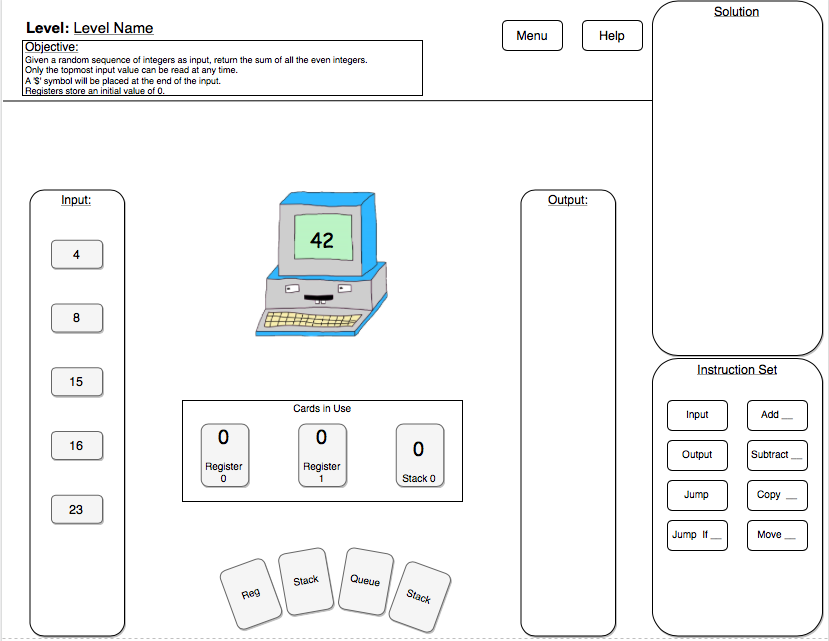
\includegraphics[scale=0.5]{Unified_Prototype.png}
\end{figure}

\begin{figure}[H]
	\caption{Unity Prototype}
	\label{fig:Unity_Prototype}
	\centering
	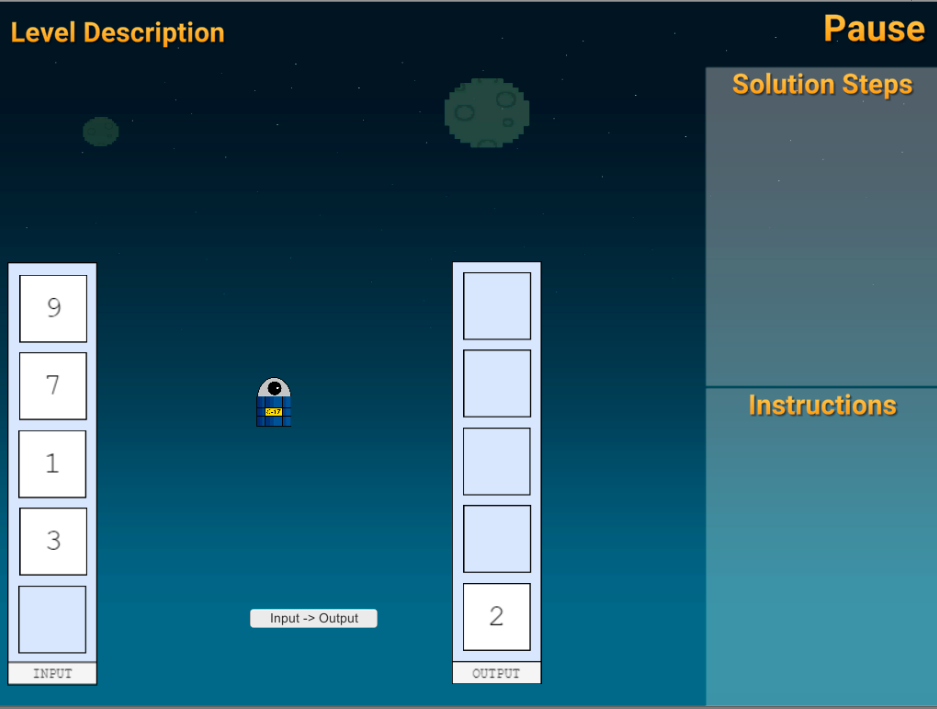
\includegraphics[scale=0.45]{Unity_Prototype.png}
\end{figure}

\subsubsection{Puzzle Scene}
\paragraph{Menu Bar:} ~\\
The menu bar spans the top of the screen of the game puzzle scene to serve as a 
container for a few other elements of the user interface.

\subparagraph{Level Description:} ~\\
The level description provides a description of the current level objectives. This 
contains text that explains the current puzzle and requirements in a concise manner. 
The level description should fit in a relatively small space, yet clearly define what is 
expected from the player. Although beginner players may get confused at certain 
points during the game, such confusion should be caused by facing unfamiliar 
Computer Science concepts, and thus alleviated by attempting the puzzles and 
observing the results. Generally players should \textit{not} be confused by what 
is expected from them, which is why the phrasing of level descriptions should be 
carefully considered and tested.

\subparagraph{Menu Button:} ~\\
The Menu button pauses the game and displays a pause menu over the puzzle scene,
 which presents the player with options to exit the puzzle scene, change certain game 
options, such as volume, and resume the game.

\subparagraph{Help Button:} ~\\
The Help button can be pressed if the player is struggling or needs help approaching 
the current puzzle. This displays relevant hints or tips for solving the puzzle so the player 
can better understand how to arrive at an appropriate solution.

\paragraph{Solution Space:} ~\\
The solution space on the right side of the screen is where players must utilize available 
instructions to construct a solution to the current puzzle. Players can drag instructions 
into the solution space, rearrange them, or remove them as they attempt to create a 
solution that satisfies the level objectives. While the player's solution is executing, the 
instruction that corresponds to the current step is highlighted to help the player understand 
what causes the actions simulated in the game space.

\paragraph{Instruction Set:} ~\\
Below the solution space on the right side of the screen is the instruction set, which 
provides all the instructions that the player can use for the current level. These instructions 
can be dragged and dropped into the solution space to construct a solution for the current 
level. The instructions do not get removed from the instruction set when the player drags 
them into the solution space, instead this creates a new instance of the instruction, so that 
a single instruction can be used multiple times in a solution. If the player clicks on an 
instruction, the description of that instruction appears on the screen to remind the player 
what the instruction does and how to use it.

\paragraph{Game Space:} ~\\
The game space is the largest element in the puzzle scene and takes up the majority of the 
total screen space, since this is where most of the action happens to visually demonstrate 
how logical instructions are executed and how the components interact. The game space 
contains a number of key components as described below.

\paragraph{Computron:} ~\\
\begin{figure}[H]
	\caption{Computron Concept Sketch}
	\label{fig:Computron_Concept_Sketch}
	\centering
	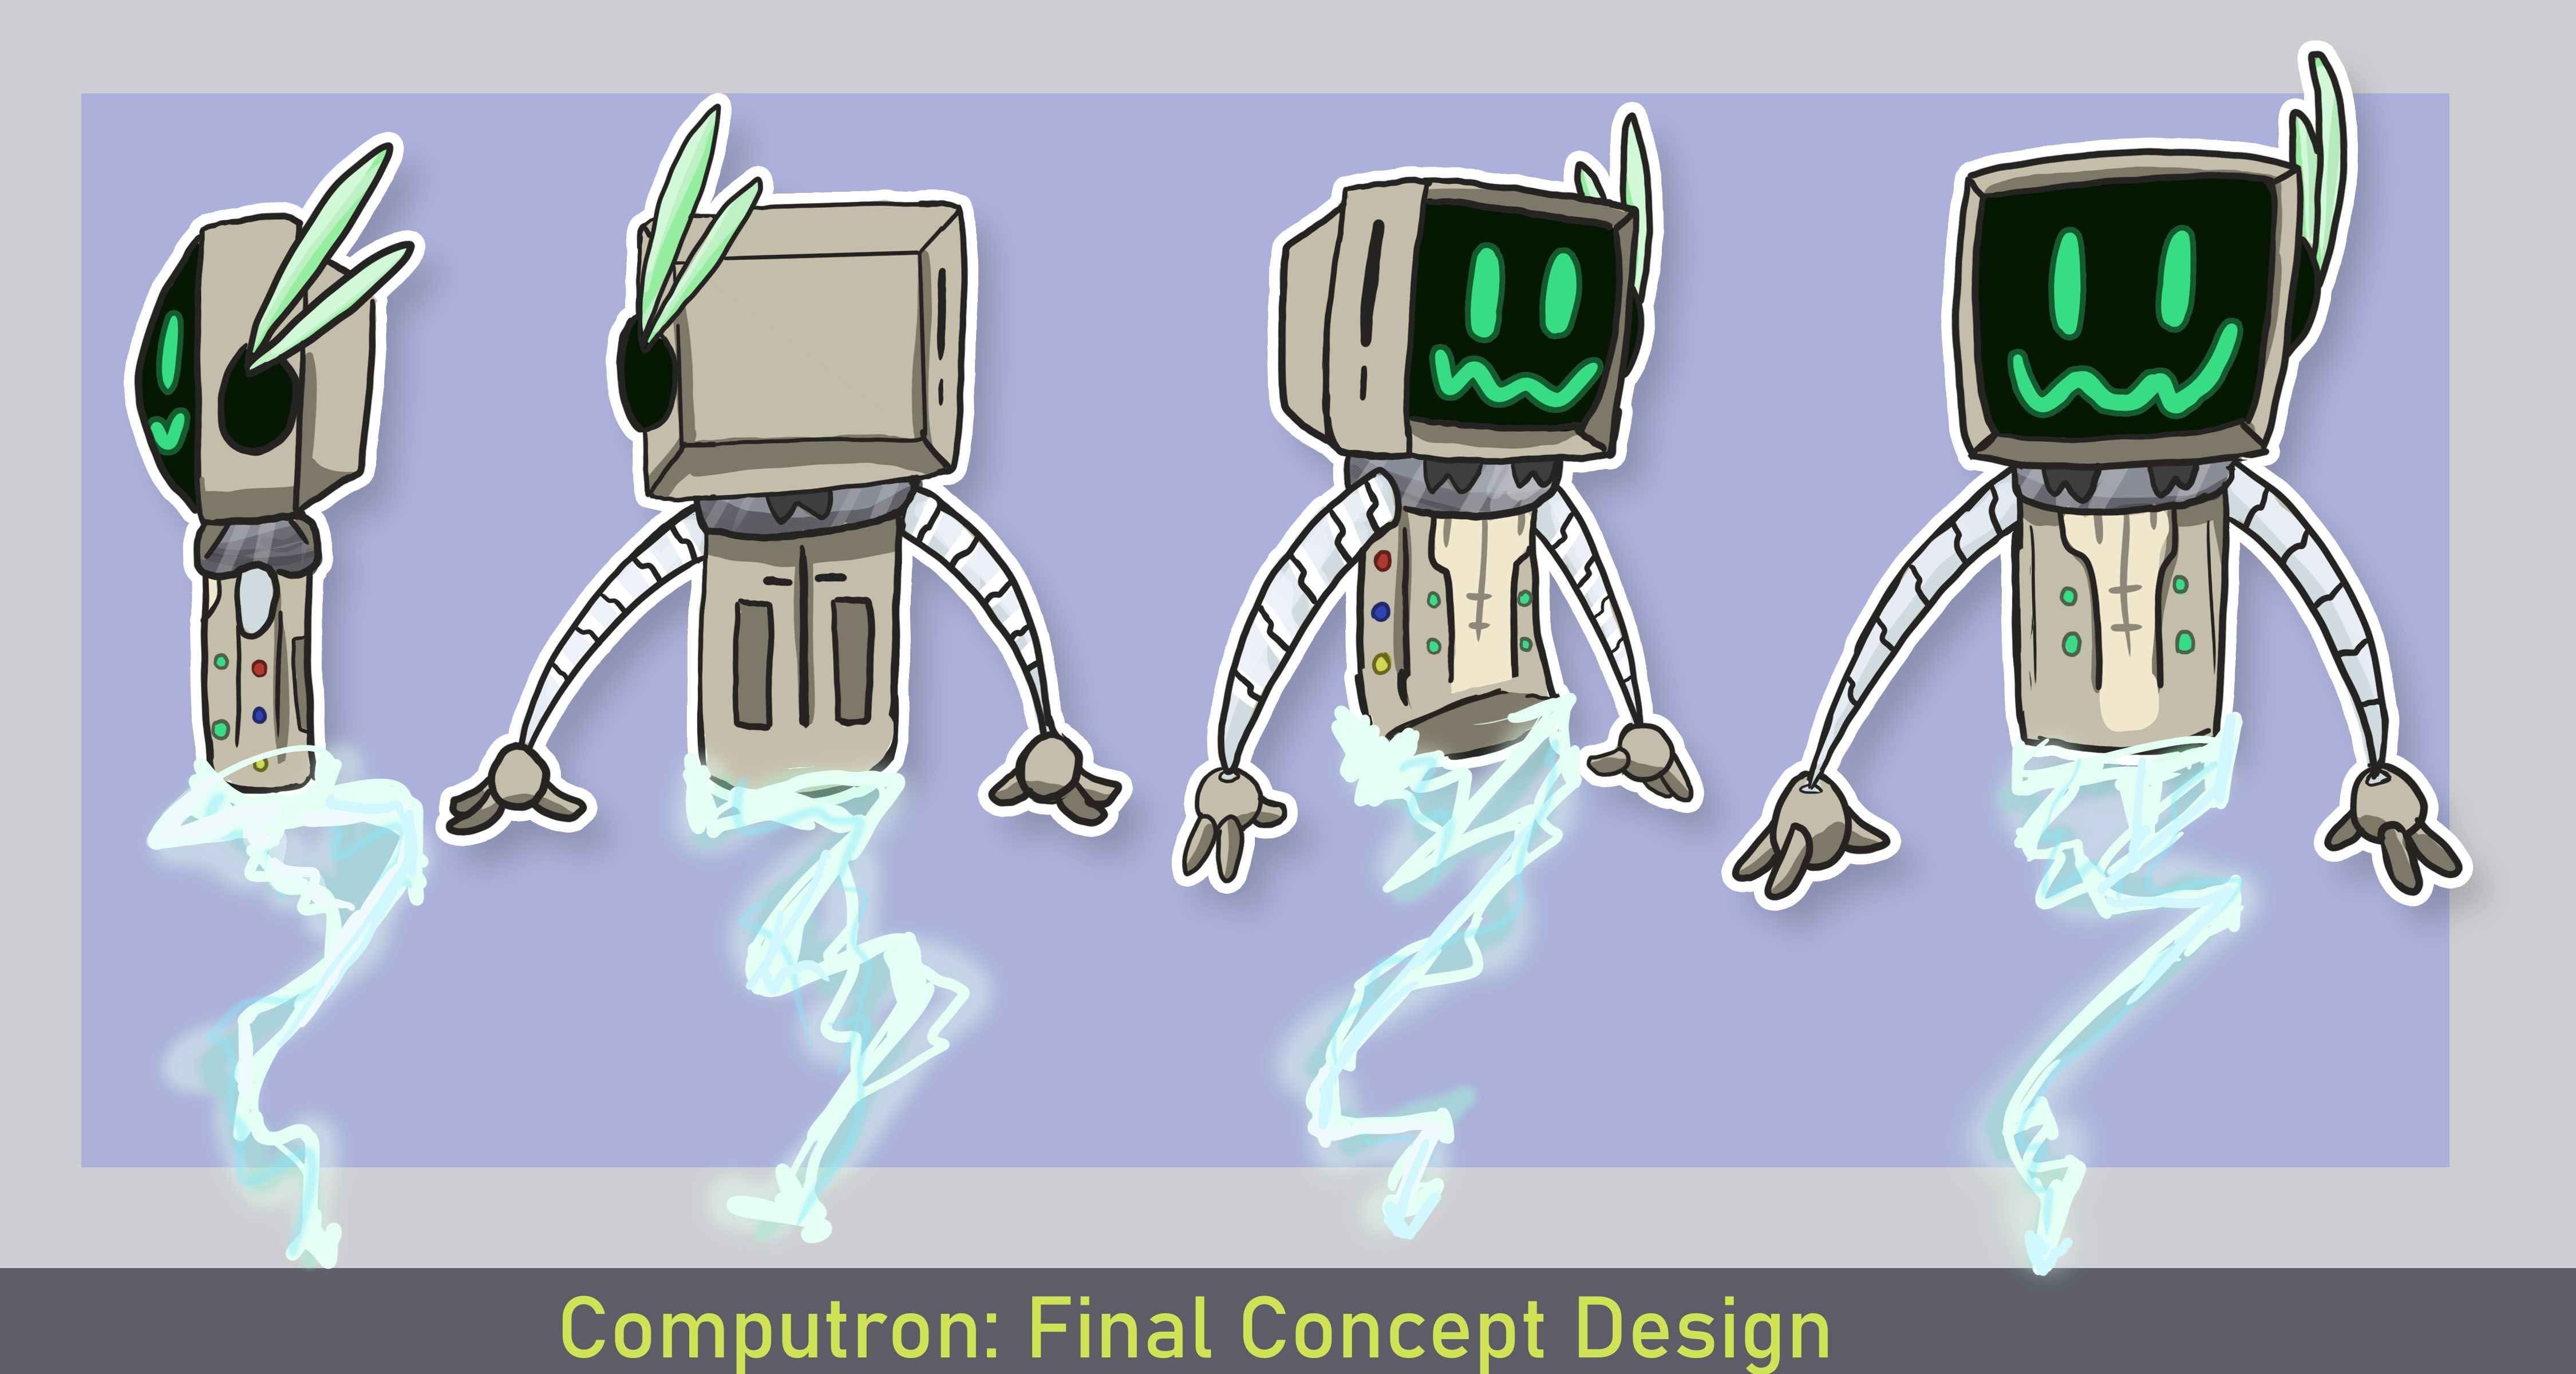
\includegraphics[scale=0.085]{ComputronFinal.jpg}
\end{figure}
The central figure of each level, Computron is the main actor for the game. Computron is 
a robotic computer character that moves around to certain components of the game space 
to simulate the steps of the player's solution. Computron can pick up input values, store 
and manipulate the data, transfer it to and from other components such as registers or data 
structures, and bring data to the output stack. Computron has a computer monitor that 
displays the current value being held, and shows changes being made to the current value.

\paragraph{Input:} ~\\
Input values are received from a vertical stack on the bottom left of the game space. This 
input stack works similarly to a conveyor belt delivering items. Computron may only pick 
up the topmost item from input, like popping a stack. When the top element of input is 
removed, the second element becomes the new top element, and all the items on the conveyor 
belt slide upwards by one space. No items can be pushed onto the input stack.

\paragraph{Output:} ~\\
Output values are delivered to a vertical stack, similar to the input stack, on the bottom right 
of the game space. When outputting a value, Computron pushes it onto the top of the output 
stack, and any items in the stack slide down by one position, and the bottom element slides 
off the screen. No items can be removed from the output once they are pushed.

\paragraph{Card Space:} ~\\
At the bottom of the game space between input and output is where data structure cards 
are stored and used. Each puzzle may include a small set of playing card objects, each 
containing a specific data structure. The possible cards are Register, Stack, Queue, and 
Heap. For the initial game state, the cards are not in use but are available to put into use if 
the player chooses. The player can do this by dragging a card from their ``hand'' up to a 
card slot above the available cards. When a card is in a slot, it becomes active and can be 
used and referenced by the instructions. Cards in use will display their contents, or if the 
data structure is too large to display, the player can click on the card  to enlarge it and view 
the current values in the data structure. Clicking on a card that is either available or in use 
also provides a description of the corresponding data structure type and how to use it.